% C.30 PA 切线, A 切点, OA=3, OP=5
\documentclass[tikz,border=4pt]{standalone}
\usepackage{ctex}
\usepackage{amsmath}
\usetikzlibrary{calc, arrows.meta}
\begin{document}
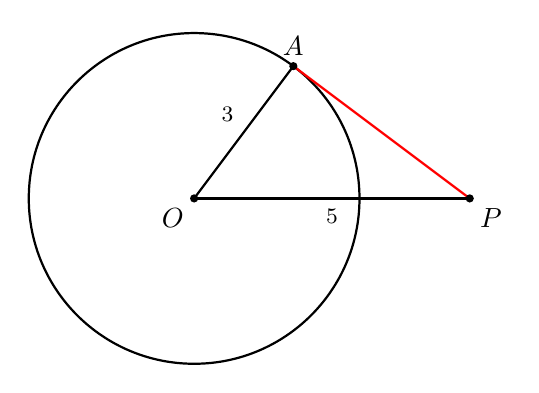
\begin{tikzpicture}[scale=0.7, thick]
  \coordinate (O) at (0,0);
  \draw (O) circle (3);
  \coordinate (P) at (5,0);
  % cos(∠AOP)=3/5 → angle = 53.13°
  \coordinate (A) at ({3*cos(53.13)},{3*sin(53.13)});
  \draw (O) -- (P);
  \draw (O) -- (A);
  \draw[red] (A) -- (P);
  \filldraw (O) circle (1.5pt) node[below left] {$O$};
  \filldraw (P) circle (1.5pt) node[below right] {$P$};
  \filldraw (A) circle (1.5pt) node[above] {$A$};
  \node[font=\footnotesize, below] at ($(O)!0.5!(P)$) {$5$};
  \node[font=\footnotesize, above left] at ($(O)!0.5!(A)$) {$3$};
\end{tikzpicture}
\end{document}
